\section{Data Acquisition}
\label{sec:chap_slam_data_acquisition}

In the following section, we first describe the robotic platform and sensors used to gather our place recognition dataset. We then describe in more details the dataset acquisition procedure and the resulting data.


\subsection{Robotic platform}
\label{ssec:chap_slam_platform}

The Husky A200 is a medium size (990 x 670 x 390 \SI{28}{\milli\meter}) \gls*{ugv} developed by \cite{ClearpathWeb}. It is a rugged robot designed for all terrain conditions, therefore well suited for our experiments in forest. It uses a differential-drive skid steer allowing easy control and in place turns for our data acquisition. It has a maximum speed of \SI{1}{\meter\per\second}, but we generally acquire data at lower speed, which minimizes odometry and range data errors. This platform, with a maximum payload capability of \SI{75}{\kilo\gram}, can easily carry all sensors used for our experiments. The platform is shown in Figure~\ref{fig:chap_slam_husky} and more details about the available devices are presented in Table~\ref{tab:husky_devices} show a list of devices available on the platform and the use we make of them.

\begin{figure}[H]
    \centering
    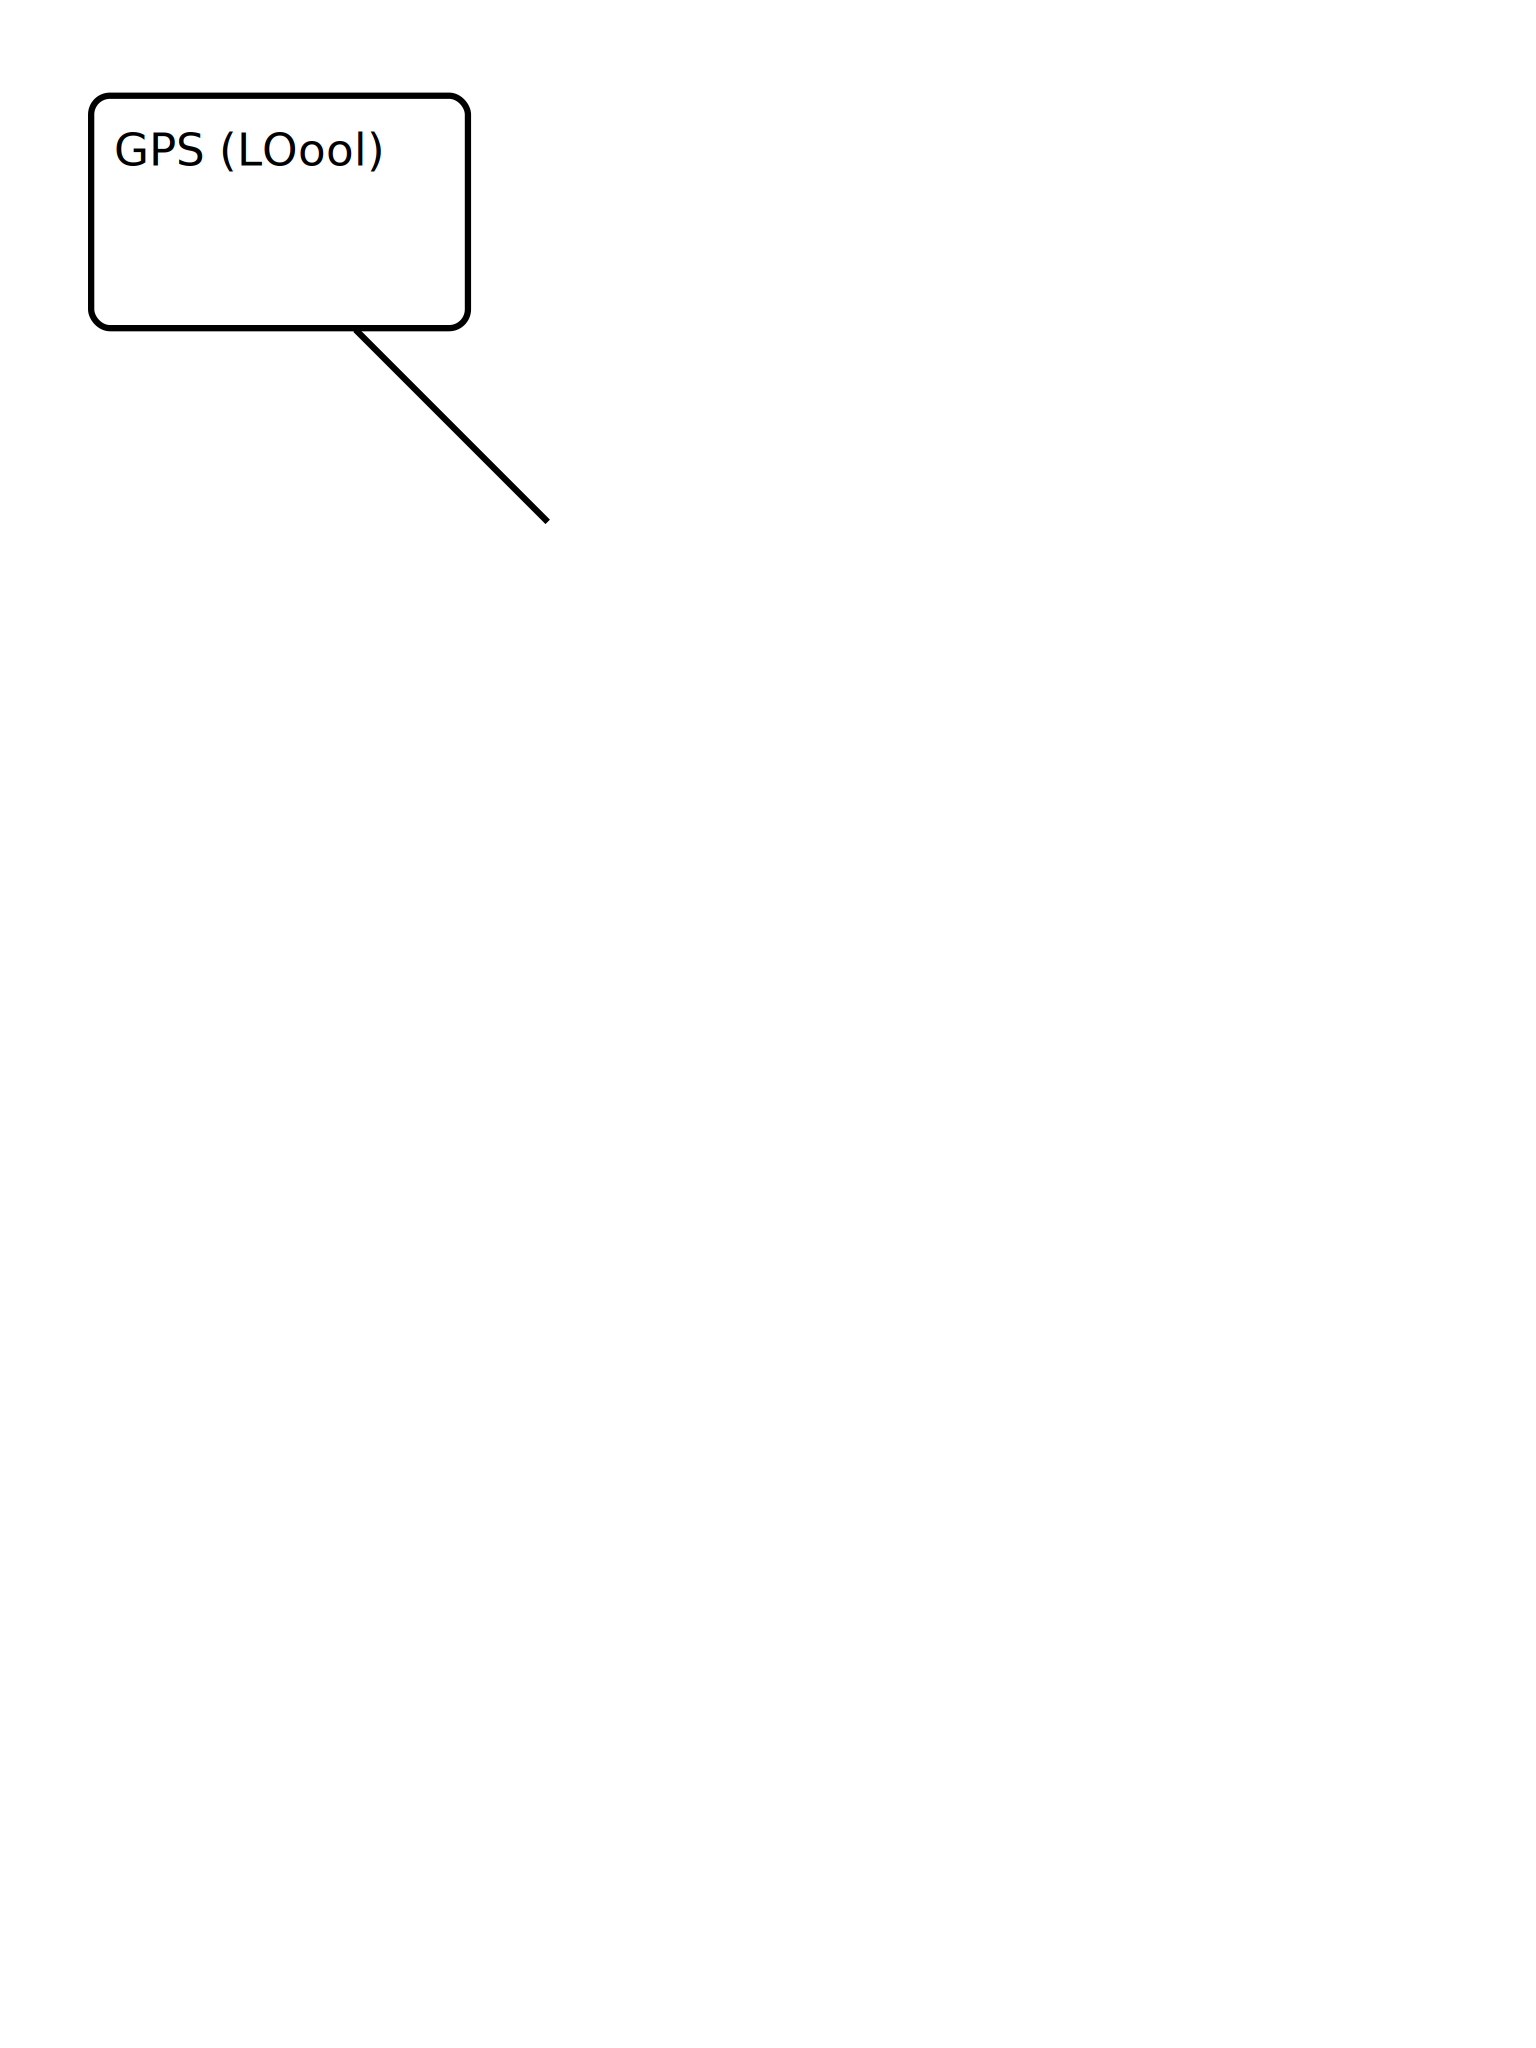
\includegraphics[width=0.98\linewidth]{img/chap_slam/husky_labelled.png}
    \caption{The robotic platform (Husky A200) and the devices used for data acquisition. The SICK \gls*{lidar} is not mounted, but is shown on the bottom right corner of the figure. Note that the \gls*{ptu} is hidden by fabric and the on-board computer is mostly occluded by the Velodyne \gls*{lidar}.}
    \label{fig:chap_slam_husky}
\end{figure}

\begin{table}[H]
    \centering
    \begin{tabular}{@{}llll@{}}
        \toprule
        \textbf{Device} & \textbf{Manufacturer}       & \textbf{Model}  & \textbf{Use}                          \\ \hline
        Computer        & --                          & --              & Data acquisition/synchronisation      \\
        Gateway         & Microhard System Inc.       & VIP2400         & Network and Wi-Fi communication       \\
        Gamepad         & Logitech                    & F710            & Remote control of the robot movements \\
        \gls*{lidar}    & Velodyne                    & HDL-32E         & Point cloud acquisition               \\
        \gls*{lidar}    & SICK                        & LMS151          & Point cloud acquisition               \\
        \gls*{ptu}      & FLIR Motion Control Systems & D46-17          & Rotate the SICK \gls*{lidar}          \\
        \gls*{imu}      & ChRobotics                  & UM6             & Odometry                              \\
        Camera          & Axis                        & M1013           & Visual reference                      \\
        \gls*{gps}      & NovAtel                     & SMART6          & Not used                              \\
        \bottomrule
    \end{tabular}
    \caption{Set of devices available on the Husky A200 and their use in our experiments. Note that both \gls*{lidar}s are not mounted at the same time.}
    \label{tab:husky_devices}
\end{table}

The on-board computer is an essential element of our experiments, as it connects all devices, acts as a control interface for the robot and stores acquired data. The computer does not provide a \gls*{gui}, but it is connected to the gateway that broadcasts a WiFi network, allowing \gls*{ssh} communication. The platform is also equipped with a wireless gamepad, which allows controlling the movements of the latter. Point clouds acquisition is possible using either the SICK LMS151 or the Velodyne HDL-32E. The selected sensor is mounted on the \gls*{ptu}, which remains fixed for the Velodyne, but is rotated with the SICK to merge multiple \gls*{2d} scans into a single \gls*{3d} point cloud. Section~\ref{ssec:chap_slam_platform} give more details about the resulting point clouds for each sensor.

The sensors described above are essential for our place recognition research, but we also use the wheel encoder along with the \gls*{imu} for odometry estimation and the camera for visual reference of the dataset. Note that we do not use the \gls*{gps}, as we do not want to depend on it for the task of place recognition.


\subsection{Dataset description}
\label{ssec:chap_slam_platform}

Data acquisition was performed using \gls*{ros}, a set of software libraries and tools created to simplify the developement in robotics. It provides all drivers for the Husky and our sensors out of the box and its data publishing system provides timestamp that allows easier synchronization between sensors. The recording tool (rosbag) was used to create our datasets and data processing was performed a posteriori.

We produced datasets on two different sites of the Laval University campus. Located between the Alexandre-Vachon and the Adrien-Pouliot buildings, the first site was chosen for its more structured nature. The environment is more open, the terrain is smooth and flat and the site contains man-made objects such as buildings, stairs or tables. \todo{Make this paragraph awesome (complete description and link the 2 sites)}. The second site, chosen for its unstructured nature, is located in a woodland of the campus. The dataset path starts on a pedestrian walkway, but after a turn of about \SI{330}{\degree}, it rolls for about \SI{100}{\meter} in rougher terrain. 

\begin{figure}[H]
    \centering
    \subfloat[]{\label{fig:path_overview}}{\includegraphics[width=0.995\linewidth]{img/chap_slam/paths.jpg}}\\ \vspace{3mm}
    \subfloat[]{\label{fig:path_building}}{\includegraphics[width=0.485\linewidth]{img/chap_slam/path_building.jpg}} \hspace{2mm}
    \subfloat[]{\label{fig:path_forest}}{\includegraphics[width=0.485\linewidth]{img/chap_slam/path_forest.jpg}}
    \caption{\protect\subref{fig:path_overview} Partial aerial view of the Laval University campus including the two approximate paths followed by the robot for data acquisition. \protect\subref{fig:path_building} Zoomed view of the path followed (counterclockwise from tag 1) in a structured environment. The length of this path is approximately \SI{160}{\meter}. \protect\subref{fig:path_forest} Zoomed view of the path followed (clockwise from tag 2) to create the forest dataset. The length of this path is approximately \SI{275}{\meter}. Images source: Google Earth, (2015)}
    \label{fig:chap_slam_path}
\end{figure}

\begin{figure}[H]
    \centering
    \subfloat[]{\label{fig:slam_view_building}}{\includegraphics[width=0.47\linewidth]{img/todo.jpg}}
    \subfloat[]{\label{fig:slam_view_forest}}{\includegraphics[width=0.47\linewidth]{img/todo.jpg}}
    \caption{Images from the \gls*{ugv} camera during the acquisition of the structured dataset \protect\subref{fig:slam_view_building} and the unstructured dataset \protect\subref{fig:slam_view_forest}. \todo{Put 2 for each ?}}
    \label{fig:slam_views}
\end{figure}

Besides the influence of the type of environment, we are also interested in the impact of the sensor used and data associated with it. For this analysis, we used two sensors, namely the SICK and the Velodyne. 

The SICK is a \gls*{2d} \gls*{lidar} with a scanning angle of \SI{270}{\degree} and a resolution of 
Information about the sensors resolution and \gls*{fov} are available in Table~\ref{tab:slam_sensor_resolution} as well as the maximum number of points in the resulting point clouds. 

Table~\ref{tab:slam_datasets} details the acquisition date and \gls*{lidar} sensor used for each of our dataset.

\begin{table}[H]
    \centering
    \begin{tabular}{@{}lrrrrr@{}}
        \toprule
    \makecell[lc]{\textbf{Sensor}}& \makecell[rc]{\textbf{Horizontal}\\\textbf{resolution}} & \makecell[rc]{\textbf{Vertical}\\\textbf{resolution}} & \makecell[rc]{\textbf{Minimum}\\\textbf{angle}} & \makecell[rc]{\textbf{Maximum}\\\textbf{angle}} & \makecell[rc]{\textbf{Points}\\\textbf{count}} \\
        \hline
        SICK LMS151      & \SI{0.57}{\degree} & \SI{0.5}{\degree}  & \SI{-45.00}{\degree}  & \SI{90.00}{\degree}  & 339120 \\
        Velodyne HDL-32E & \SI{0.16}{\degree} & \SI{1.33}{\degree} & \SI{-30.68}{\degree}  & \SI{10.67}{\degree}  & 72000  \\
        \bottomrule
    \end{tabular}
    \caption{Details about the point clouds created with our two \gls*{lidar}s. The minimum and maximum angles are given relative to an horizontal plane in the sensor frame of reference and both sensor report \SI{360}{\degree} around the vertical axis. The points count represent the maximum number of points in the resulting point cloud  }
    \label{tab:slam_sensor_resolution}
\end{table}

\begin{table}[H]
    \centering
    \begin{tabular}{@{}lll@{}}
        \toprule
        \textbf{Site}  & \textbf{Sensor}   & \textbf{Date}                     \\
        \hline
        Structured     & SICK LMS151       & July 16\textsuperscript{th}, 2015 \\
        Unstructured   & SICK LMS151       & July 14\textsuperscript{th}, 2015 \\
        Unstructured   & Velodyne HDL-32E  & May 28\textsuperscript{th}, 2015  \\
        \bottomrule
    \end{tabular}
    \caption{Datasets acquired for place recognition analysis.}
    \label{tab:slam_datasets}
\end{table}

\begin{figure}[H]
    \centering
    \subfloat[]{\label{fig:slam_pointcloud_building}}{\includegraphics[width=0.47\linewidth]{img/todo.jpg}}
    \subfloat[]{\label{fig:slam_pointcloud_forest}}{\includegraphics[width=0.47\linewidth]{img/todo.jpg}}
    \caption{\todo{do me}}
    \label{fig:slam_pointclouds}
\end{figure}

\begin{itemize}
    \item SICK LMS151 vs velodyne (only in forest, angles/density, show point clouds side by side in a figure.)
    \item Talk about the odometry information and the correction using ICP
    \item SICK 270 degree angle at resolution of 0.5 degree for 540 points with frequency of 50hz. Pan: speed 0.25 rad/sec for 3.14 rad = 628 scans
    \item For a maximum of $3.14*4*50*540=339120$ points
    \item Velodyne (note that because of udp streaming, variable rotation speed\dots points count might change.)
    \item 32 rings distributed evenly from -30.67 to 10.67 and turn 360 degrees.
    \item According to the datasheet: 700000 points/second at 10hz = 70000 points/cloud
    \item 600 rpm for around 0.16 degrees = 72000 points /cloud
\end{itemize}

